\documentclass{ximera}
\graphicspath{  %% When looking for images,
{./}            %% look here first,
{./pictures/}   %% then look for a pictures folder,
{../pictures/}  %% which may be a directory up.
{../../pictures/}  %% which may be a directory up.
{../../../pictures/}  %% which may be a directory up.
{../../../../pictures/}  %% which may be a directory up.
}

\usepackage{listings}
%\usepackage{circuitikz}
\usepackage{xcolor}
\usepackage{amsmath,amsthm}
\usepackage{subcaption}
\usepackage{graphicx}
\usepackage{tikz}
%\usepackage{tikz-3dplot}
\usepackage{amsfonts}
%\usepackage{mdframed} % For framing content
%\usepackage{tikz-cd}

  \renewcommand{\vector}[1]{\left\langle #1\right\rangle}
  \newcommand{\arrowvec}[1]{{\overset{\rightharpoonup}{#1}}}
  \newcommand{\ro}{\texttt{R}}%% row operation
  \newcommand{\dotp}{\bullet}%% dot product
  \renewcommand{\l}{\ell}
  \let\defaultAnswerFormat\answerFormatBoxed
  \usetikzlibrary{calc,bending}
  \tikzset{>=stealth}
  




%make a maroon color
\definecolor{maroon}{RGB}{128,0,0}
%make a dark blue color
\definecolor{darkblue}{RGB}{0,0,139}
%define the color fourier0 to be the maroon color
\definecolor{fourier0}{RGB}{128,0,0}
%define the color fourier1 to be the dark blue color
\definecolor{fourier1}{RGB}{0,0,139}
%define the color fourier 1t to be the light blue color
\definecolor{fourier1t}{RGB}{173,216,230}
%define the color fourier2 to be the dark green color
\definecolor{fourier2}{RGB}{0,100,0}
%define teh color fourier2t to be the light green color
\definecolor{fourier2t}{RGB}{144,238,144}
%define the color fourier3 to be the dark purple color
\definecolor{fourier3}{RGB}{128,0,128}
%define the color fourier3t to be the light purple color
\definecolor{fourier3t}{RGB}{221,160,221}
%define the color fourier0t to be the red color
\definecolor{fourier0t}{RGB}{255,0,0}
%define the color fourier4 to be the orange color
\definecolor{fourier4}{RGB}{255,165,0}
%define the color fourier4t to be the darker orange color
\definecolor{fourier4t}{RGB}{255,215,0}
%define the color fourier5 to be the yellow color
\definecolor{fourier5}{RGB}{255,255,0}
%define the color fourier5t to be the darker yellow color
\definecolor{fourier5t}{RGB}{255,255,100}
%define the color fourier6 to be the green color
\definecolor{fourier6}{RGB}{0,128,0}
%define the color fourier6t to be the darker green color
\definecolor{fourier6t}{RGB}{0,255,0}

%New commands for this doc for errors in copying
\newcommand{\eigenvar}{\lambda}
%\newcommand{\vect}[1]{\mathbf{#1}}
\renewcommand{\th}{^{\text{th}}}
\newcommand{\st}{^{\text{st}}}
\newcommand{\nd}{^{\text{nd}}}
\newcommand{\rd}{^{\text{rd}}}
\newcommand{\paren}[1]{\left(#1\right)}
\newcommand{\abs}[1]{\left|#1\right|}
\newcommand{\R}{\mathbb{R}}
\newcommand{\C}{\mathbb{C}}
\newcommand{\Hilb}{\mathbb{H}}
\newcommand{\qq}[1]{\text{#1}}
\newcommand{\Z}{\mathbb{Z}}
\newcommand{\N}{\mathbb{N}}
\newcommand{\q}[1]{\text{``#1''}}
%\newcommand{\mat}[1]{\begin{bmatrix}#1\end{bmatrix}}
\newcommand{\rref}{\text{reduced row echelon form}}
\newcommand{\ef}{\text{echelon form}}
\newcommand{\ohm}{\Omega}
\newcommand{\volt}{\text{V}}
\newcommand{\amp}{\text{A}}
\newcommand{\Seq}{\textbf{Seq}}
\newcommand{\Poly}{\textbf{P}}
\renewcommand{\quad}{\text{    }}
\newcommand{\roweq}{\simeq}
\newcommand{\rowop}{\simeq}
\newcommand{\rowswap}{\leftrightarrow}
\newcommand{\Mat}{\textbf{M}}
\newcommand{\Func}{\textbf{Func}}
\newcommand{\Hw}{\textbf{Hamming weight}}
\newcommand{\Hd}{\textbf{Hamming distance}}
\newcommand{\rank}{\text{rank}}
\newcommand{\longvect}[1]{\overrightarrow{#1}}
% Define the circled command
\newcommand{\circled}[1]{%
  \tikz[baseline=(char.base)]{
    \node[shape=circle,draw,inner sep=2pt,red,fill=red!20,text=black] (char) {#1};}%
}

% Define custom command \strikeh that just puts red text on the 2nd argument
\newcommand{\strikeh}[2]{\textcolor{red}{#2}}

% Define custom command \strikev that just puts red text on the 2nd argument
\newcommand{\strikev}[2]{\textcolor{red}{#2}}

%more new commands for this doc for errors in copying
\newcommand{\SI}{\text{SI}}
\newcommand{\kg}{\text{kg}}
\newcommand{\m}{\text{m}}
\newcommand{\s}{\text{s}}
\newcommand{\norm}[1]{\left\|#1\right\|}
\newcommand{\col}{\text{col}}
\newcommand{\sspan}{\text{span}}
\newcommand{\proj}{\text{proj}}
\newcommand{\set}[1]{\left\{#1\right\}}
\newcommand{\degC}{^\circ\text{C}}
\newcommand{\centroid}[1]{\overline{#1}}
\newcommand{\dotprod}{\boldsymbol{\cdot}}
%\newcommand{\coord}[1]{\begin{bmatrix}#1\end{bmatrix}}
\newcommand{\iprod}[1]{\langle #1 \rangle}
\newcommand{\adjoint}{^{*}}
\newcommand{\conjugate}[1]{\overline{#1}}
\newcommand{\eigenvarA}{\lambda}
\newcommand{\eigenvarB}{\mu}
\newcommand{\orth}{\perp}
\newcommand{\bigbracket}[1]{\left[#1\right]}
\newcommand{\textiff}{\text{ if and only if }}
\newcommand{\adj}{\text{adj}}
\newcommand{\ijth}{\emph{ij}^\text{th}}
\newcommand{\minor}[2]{M_{#2}}
\newcommand{\cofactor}{\text{C}}
\newcommand{\shift}{\textbf{shift}}
\newcommand{\startmat}[1]{
  \left[\begin{array}{#1}
}
\newcommand{\stopmat}{\end{array}\right]}
%a command to give a name to explorations and hints and theorems
\newcommand{\name}[1]{\begin{centering}\textbf{#1}\end{centering}}
\newcommand{\vect}[1]{\vec{#1}}
\newcommand{\dfn}[1]{\textbf{#1}}
\newcommand{\transpose}{\mathsf{T}}
\newcommand{\mtlb}[2][black]{\texttt{\textcolor{#1}{#2}}}
\newcommand{\RR}{\mathbb{R}} % Real numbers
\newcommand{\id}{\text{id}}
\newcommand{\coord}[1]{\langle#1\rangle}
\newcommand{\RREF}{\text{RREF}}
\newcommand{\Null}{\text{Null}}
\newcommand{\Nullity}{\text{Nullity}}
\newcommand{\Rank}{\text{Rank}}
\newcommand{\Col}{\text{Col}}
\newcommand{\Ef}{\text{EF}}
\newcommand{\boxprod}[3]{\abs{(#1\times#2)\cdot#3}}

\author{Zack Reed}
%borrowed from selinger linear algebra
\title{Linear Combination, Span, and Bases}
\begin{document}
\begin{abstract}

\end{abstract}
\maketitle

Let's think about two vectors, $\vect{u}$ and $\vect{v}$ in $\R^n$. In the previous chapter, we noted that \emph{linear combinations} provide the fundamental operations on vectors in Linear Algebra. In fact, most of waht we will discuss in this course will be based on linear combinations, structured in certain ways.

\begin{exploration}\name{Span}

One very important way of thinking about how vectors relate to each other is to consider their \emph{span}.


\begin{definition}\name{Span of a set of vectors}
  The set of all linear combinations of the vectors
  $\vect{u}_1, \ldots,\vect{u}_k$ in $\R^n$ is known as the
  \textbf{span}%
  \index{span}%
  \index{vector!span} of these vectors and is written as
  $\sspan\set{\vect{u}_1,\ldots,\vect{u}_k}$. Using set notation, we
  can write
  \begin{equation*}
    \sspan\set{\vect{u}_1,\ldots,\vect{u}_k}
    ~=~ \set{a_1\vect{u}_1+\ldots+a_k\vect{u}_k \mid a_1,\ldots,a_k\text{ in }\R}.
  \end{equation*}
  \begin{hint}\name{{\bf Hint: Notation Alert!}}
  
    Set notation is a common and succinct way to describe collections of mathematical objects. Learning to read set-notation is important for being increasingly comfortable with the language of mathematics as it applies to the sciences.

    The notation $\set{a_1\vect{u}_1+\ldots+a_k\vect{u}_k \mid a_1,\ldots,a_k\text{ in }\R}$ reads "all new vectors $\vect{v}$ of the form $a_1\vect{u}_1+\ldots+a_k\vect{u}_k$ where $a_1,\ldots,a_k$ are real numbers." In words we would say this is all possible linear combinations of the vectors $\vect{u}_1,\ldots,\vect{u}_k$, since we're allowing any collection of real nubmers to scale and add the vectors together.

  \end{hint}
\end{definition}

We can picture the set of their linear combinations as follows:
\begin{center}
  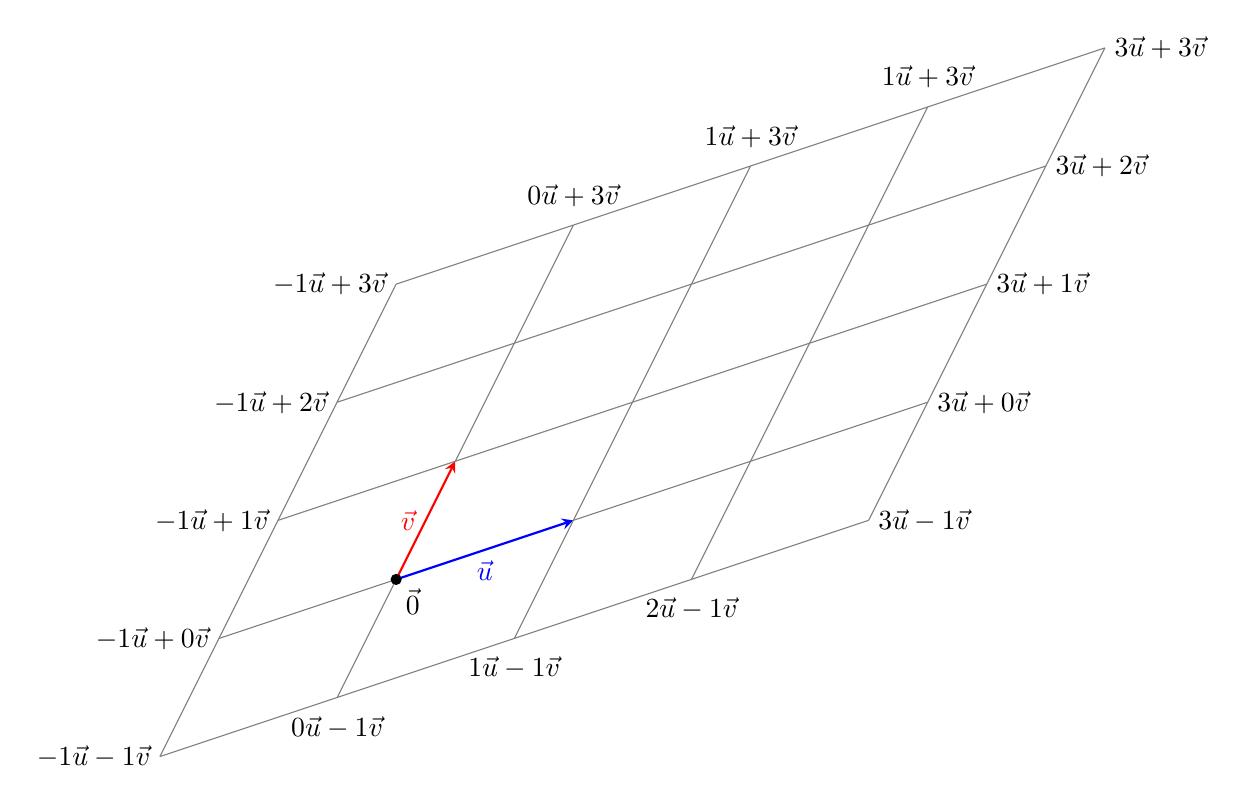
\begin{tikzpicture}[scale=1.5]
    \draw[->, thick, blue] (0,0) -- node[below]{$\vect{u}$} (1.5,0.5);
    \draw[->, thick, red] (0,0) -- node[left]{$\vect{v}$} (0.5,1);
    \draw[-, gray] (-2,-1.5)--(4,0.5);
    \draw[-, gray] (-1.5,-0.5)--(0,0);
    \draw[-, gray] (1.5,0.5)--(4.5,1.5);
    \draw[-, gray] (-1,0.5)--(5,2.5);
    \draw[-, gray] (-0.5,1.5)--(5.5,3.5);
    \draw[-, gray] (0,2.5)--(6,4.5);
    \draw[-, gray] (-2,-1.5)--(0,2.5);
    \draw[-, gray] (-0.5,-1)--(0,0);
    \draw[-, gray] (0.5,1)--(1.5,3);
    \draw[-, gray] (1,-0.5)--(3,3.5);
    \draw[-, gray] (2.5,0)--(4.5,4);
    \draw[-, gray] (4,0.5)--(6,4.5);
    \draw (-2.0,-1.5) node[left]{$-1\vect{u}-1\vect{v}$};
    \draw (-1.5,-0.5) node[left]{$-1\vect{u}+0\vect{v}$};
    \draw (-1.0,0.5) node[left]{$-1\vect{u}+1\vect{v}$};
    \draw (-0.5,1.5) node[left]{$-1\vect{u}+2\vect{v}$};
    \draw (0.0,2.5) node[left]{$-1\vect{u}+3\vect{v}$};
    \draw (1.5,3.0) node[above=0.75ex]{$0\vect{u}+3\vect{v}$};
    \draw (3.0,3.5) node[above=0.75ex]{$1\vect{u}+3\vect{v}$};
    \draw (4.5,4.0) node[above=0.75ex]{$1\vect{u}+3\vect{v}$};
    \draw (6.0,4.5) node[right]{$3\vect{u}+3\vect{v}$};
    \draw (5.5,3.5) node[right]{$3\vect{u}+2\vect{v}$};
    \draw (5.0,2.5) node[right]{$3\vect{u}+1\vect{v}$};
    \draw (4.5,1.5) node[right]{$3\vect{u}+0\vect{v}$};
    \draw (4.0,0.5) node[right]{$3\vect{u}-1\vect{v}$};
    \draw (2.5,0.0) node[below=0.75ex]{$2\vect{u}-1\vect{v}$};
    \draw (1.0,-0.5) node[below=0.75ex]{$1\vect{u}-1\vect{v}$};
    \draw (-0.5,-1.0) node[below=0.75ex]{$0\vect{u}-1\vect{v}$};
    \draw[fill] (0,0) circle [radius=1.2pt] node[below right]{$\vect{0}$};
  \end{tikzpicture}
\end{center}

As the picture shows, the linear combinations of $\vect{u}$ and
$\vect{v}$ form a \emph{$2$-dimensional plane} through the origin. We say
that this plane is \textbf{spanned}%
\index{span}%
\index{vector!span} by the vectors $\vect{u}$ and $\vect{v}$. 

\begin{remark}

If you're not familiar with planes from previous courses, think of a flat sheet of paper cutting through 3-D space. We'll make this more sophisticated in later chapters, but for now we're only going to define planes in terms of span, below.

\end{remark}

This
concept generalizes to more than two vectors. For example, three
vectors may span a $3$-dimensional space (or sometimes a $2$-dimensional space, a line, or just the origin). We'll dig into this more in the next exploration, for now let's just work with the span of a couple of vectors.

\end{exploration}

\begin{exploration}\name{Span in $\R^2$ and $\R^3$}

Let's start by looking in $\R^2$. The following GeoGebra applet allows you to input two vectors and see their span in $\R^2$. 

You can select the appropriate boxes to set the spanning vectors, and then click the "Show Span" button to see the span. You can then drag the vector $\vect{v}$ to see the linear combination of the spanning vectors that make up $\vect{v}$.

\begin{example}

  Using the applet, set $\vect{u}=\startmat{r} 1 \\ 1 \stopmat$ and $\vec{w}=\startmat{r} 2 \\ 3 \stopmat$. Then click "Show Span" to see the span of these vectors in $\R^2$.

  \begin{center}
    \geogebra{rfbeefhu}{846}{503}
  \end{center}

  Select the "Standard Span" button and drag the vector $\vec{v}$ to $\vec{v}=[1,2]$. If you then check the "See New Span" box, the grid will shift to the span of your two vectors. 
  
  Using the applet, what linear combination of $\vec{u}$ and $\vec{w}$ makes up $\vec{v}$?

  \begin{hint}\name{{\bf Hint:}}
  
    Remember that a negative scalar multiple of a vector poitns in the opposite direction of the vector.

  \end{hint}

  \begin{solution}
  
    $\vec{v}=\answer{-1}\vec{u}+\answer{1}\vec{w}$.

  \end{solution}

\end{example}

\begin{example}\name{Spanning Multiple Vectors}

  Now, use the applet to find the linear combinations of the vectors $\vec{u}$ and $\vec{w}$ that make up the vectors $\vec{v}$:

  \begin{enumerate}
  
    \item $\vec{u}=[1,2]$, $\vec{w}=[2,1]$, 
    
    $$\answer{2}\vec{u}+\answer{1}\vec{w}=[4,5].$$

    \item $\vec{u}=[1,2]$, $\vec{w}=[-2,1]$,
    
    $$\answer{-1}\vec{u}+\answer{3}\vec{w}=[-7,1].$$

  \end{enumerate}

\end{example}

\begin{example}\name{Vectors in a span}
  Let $\vect{u}=\startmat{r} 1 \\ 1 \\ 1 \stopmat$ and
  $\vect{v}=\startmat{r} 3 \\ 2 \\ 1 \stopmat$. Which
  of the following vectors are elements of
  $\sspan\set{\vect{u},\vect{v}}$?
  \begin{equation*}
    (a)\quad\vect{w} = \startmat{r} 2 \\ 3 \\ 4 \stopmat,
    \qquad
    (b)\quad\vect{z} = \startmat{r} 1 \\ 1 \\ 2 \stopmat.
  \end{equation*}

  \begin{hint}
  
    Remember that to be in $\sspan{\vect{u},\vect{v}}$, a vector must be a linear combination of $\vect{u}$ and $\vect{v}$.

  \end{hint}

  \begin{solution}

  Before we work it out analytically, let's visualize this example in GeoGebra. The following applet lets you input three vectors to view their span in $\R^3$.

  You can select the appropriate boxes to set the spanning vectors, and then click the "Show Span" button to see the span. You can then drag the vector $\vect{v}$ to see whether or not it is in the span of the vectors.

  Since the applet requires 3 vectors, for this example input $\vec{u}, \vec{v}, \vec{w}$. 

  \begin{center}
    \geogebra{y95ydrhy}{798}{478}
  \end{center}

  Notice that the span of $\vect{u}$ and $\vect{v}$ is a plane, and that $\vect{w}$ is in this plane, while $\vect{z}$ is not.

\end{solution}

  \begin{solution}
    (a) For a vector to be in $\sspan\set{\vect{u},\vect{v}}$, it must
    be a linear combination of $\vect{u}$ and $\vect{v}$. Therefore,
    $\vect{w}\in\sspan\set{\vect{u},\vect{v}}$ if and only if we can
    find find scalars $a,b$ such that
    $a\,\vect{u} + b\,\vect{v} = \vect{w}$. We must therefore solve the
    equation
    \begin{equation*}
      a \startmat{r} 1 \\ 1 \\ 1 \stopmat
      + b \startmat{r} 3 \\ 2 \\ 1 \stopmat
      = \startmat{r} 2 \\ 3 \\ 4 \stopmat.
    \end{equation*}
   
    If we take each component individually, this gives us the system of equations
    \begin{equation*}
      \begin{array}{r@{~}c@{~}r@{~}c@{~}r@{~}r}
        a & + & 3b & = & 2, \\
        a & + & 2b & = & 3, \\
        a & + & b & = & 4.
      \end{array}
    \end{equation*}

    We solve this by isolating $a$ in the last equation: 

    \begin{equation*}
      a = 4 - b.
    \end{equation*}

    Substituting this into the first equation gives us

    \begin{equation*}
      4 - b + 3b = 2 \quad \Rightarrow \quad 4 + 2b = 2 \quad \Rightarrow \quad 2b = -2 \quad \Rightarrow \quad b = -1.
    \end{equation*}

    We then substitute back into the third equation to find $a$:

    \begin{equation*}
      a = 4 - (-1) = 5.
    \end{equation*}

    Luckily, this solution works in the second equation as well:

    \begin{equation*}
      5 + 2(-1) = 3.
    \end{equation*}
  
    The solution is $a=5$ and $b=-1$. This means that
    $\vect{w} = 5\vect{u} + (-1)\vect{v}$. Therefore, $\vect{w}$ is an
    element of $\sspan\set{\vect{u},\vect{v}}$.
  
    (b) If we try the same approach with $\vect{z}$, we get the system of equations
  
    \begin{equation*}
      \begin{array}{r@{~}c@{~}r@{~}c@{~}r@{~}r}
        a & + & 3b & = & 1, \\
        a & + & 2b & = & 1, \\
        a & + & b & = & 2.
      \end{array}
    \end{equation*}

    Again isolating $a$ in the last equation gives us

    \begin{equation*}
      a = 2 - b.
    \end{equation*}

    Substituting this into the first equation gives us

    \begin{equation*}
      2 - b + 3b = 1 \quad \Rightarrow \quad 2 + 2b = 1 \quad \Rightarrow \quad 2b = -1 \quad \Rightarrow \quad b = -\frac{1}{2}.
    \end{equation*}

    We then substitute back into the third equation to find $a$:

    \begin{equation*}
      a = 2 - \left(-\frac{1}{2}\right) = \frac{5}{2}.
    \end{equation*}

    Substituting these values back into the second equation gives us

    \begin{equation*}
      \frac{5}{2} + 2\left(-\frac{1}{2}\right) = \frac{3}{2}\neq 1.
    \end{equation*}

    So $a=\frac{5}{2}$ and $b=-\frac{1}{2}$ do not satisfy the second equation.

    Since our $a$ and $b$ can't satisfy all three equations at once, there is no solution. We conclude
    that $\vect{z}$ is not an element of
    $\sspan\set{\vect{u},\vect{v}}$.
  \end{solution}

  \begin{solution}
  
    One final time, let's solve this problem, but with MATLAB. 

    MATLAB provides a fast way to solve systems of equations and vector equations, using the $\texttt{solve}$ function.

    First set up your vectors:
\begin{verbatim}
u=[1,1,1]
v=[3, 2, 1]
w=[2, 3, 4]
z=[1,1,2]
\end{verbatim}

Then set up the variables for the unknown coefficients:
\begin{verbatim}
syms a b
\end{verbatim}

Also assume that their square sum is not zero, so that we ignore any trivial results like \(0 + 0 = 0\):
\begin{verbatim}
assume(a^2+b^2>0)
\end{verbatim}

First check \verb|u|, \verb|v|, and \verb|w|, setting up the linear combination. We use \verb|==| because \verb|=| is used for naming:
\begin{verbatim}
vector_equation = a*u + b*v == w
\end{verbatim}

Solve for the \verb|a| and \verb|b| if they exist:
\begin{verbatim}
solve(vector_equation, [a,b])
\end{verbatim}

Now try \verb|u|, \verb|v|, and \verb|z|:
\begin{verbatim}
vector_equation_2 = a*u + b*v == z
solve(vector_equation_2, [a,b])
\end{verbatim}

There's no solution, so \verb|z| is not in the span of \verb|u| and \verb|v|.


  \end{solution}
  
\end{example}

\end{exploration}

\begin{exploration}\name{Redundant Vectors, Lines, and Planes}

  In the previous example, we saw that the span of the three vectors $\vect{u}$, $\vect{v}$, and $\vect{w}$ in $\R^3$ was not enough to reach $\vec{z}$. More generally, the span of these three vectors can at most reach the plane spanned by $\vect{u}$ and $\vect{v}$, and so we would say that $\vect{w}$ is \emph{redundant} in this case.

  The issue of redundancy means that even if you have $n$ vectors in $\R^n$, they may not be enough to span all of $\R^n$. In fact, a collection of vectors might only span any $k$-dimensional space within $\R^n$, where $k$ is less than or equal to $n$.

  This motivates the following definitions of lines, planes, and what are called \emph{hyperplanes} in $\R^n$.

  \begin{remark}

    We now come to definitions of common spaces of vectors that you will encounter, \emph{lines, planes}, and \emph{hyperplanes}. You've at least encountered lines in previous classes, and they will have been defined differently than what you see here. We will cover lines and planes more fully in Chapter 5, and will align the notion of linear spaces to those encountered in past courses.

  \end{remark}

  \begin{definition}\name{Lines}

    A \textbf{line} in $\R^n$ is the span of one vectors $\vect{u}$ in $\R^n$. 
    
    Since linear combinations of a single vector are just scalar multiples of that vector, the line is the set of all scalar multiples of $\vect{u}$, and is written as $\sspan\set{\vect{u}}=\set{a\vect{u}\mid a\text{ in }\R}$.

  \end{definition}

  \begin{definition}\name{Planes}

    A \textbf{plane} in $\R^n$ is the span of two  non-redundant vectors $\vect{u}$ and $\vect{v}$ in $\R^n$. 
    
    Planes are written as $\sspan\set{\vect{u},\vect{v}}=\set{a\vect{u}+b\vect{v}\mid a,b\text{ in }\R}$.

  \end{definition}

  \begin{definition}\name{Hyperplanes}

    A \textbf{hyperplane} in $\R^n$ is the span of $k$ non-redundant vectors in $\R^n$, where $k< n$. 
    
    Hyperplanes are written as 
    
    $$\sspan\set{\vect{u}_1,\ldots,\vect{u}_{n-1}}=\set{a_1\vect{u}_1+\ldots+a_{n-1}\vect{u}_{n-1}\mid a_1,\ldots,a_{n-1}\text{ in }\R}.$$

  \end{definition}

  You can visualize at least the constructions of lines and planes from spans in $\R^2$ and $\R^3$, and to be exhaustive let's also consider the span of 0 vectors.

  \begin{center}
    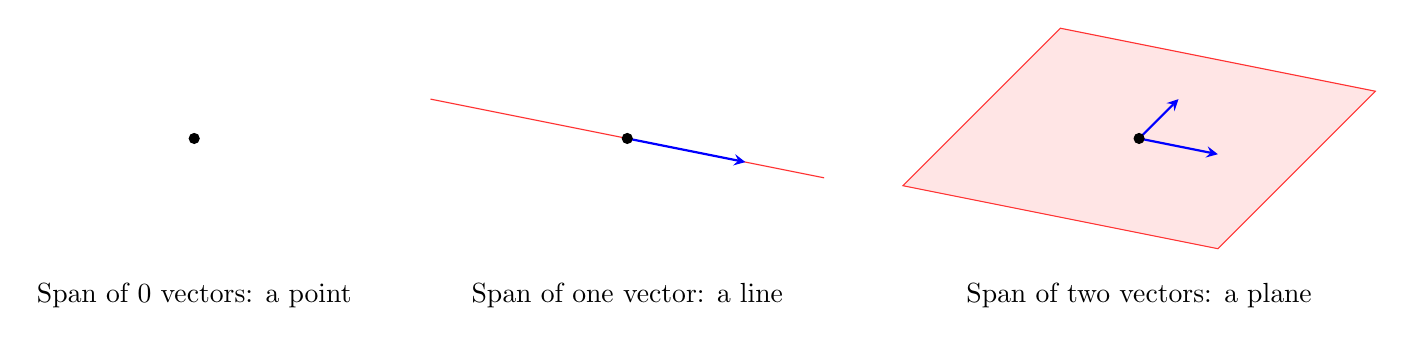
\begin{tikzpicture}
      \begin{scope}[xshift=-6cm]
        \draw[fill](0,0) circle [radius=1.8pt];
        \path(0,-2) node {Span of 0 vectors: a point};
      \end{scope}
      \begin{scope}[xshift=-0.5cm]
        \begin{scope}[x={(1cm,-0.2cm)},y={(0.5cm,0.5cm)}]
          \draw[red!80](-2.5,0) -- (2.5,0);
          \draw[->, thick, blue](0,0) -- +(1.5,0);
          \draw[fill](0,0) circle [radius=1.8pt];
        \end{scope}
        \path(0,-2) node {Span of one vector: a line};
      \end{scope}
      \begin{scope}[xshift=6cm]
        \begin{scope}[x={(1cm,-0.2cm)},y={(0.5cm,0.5cm)},z={(0cm,1cm)}]
          \filldraw[draw=red!80,fill=red!10](-2,-2,0) -- (2,-2,0) -- (2,2,0) -- (-2,2,0) -- cycle;
          \draw[->, thick, blue](0,0) -- +(0,1,0);
          \draw[->, thick, blue](0,0,0) -- +(1,0,0);
          \draw[fill](0,0) circle [radius=1.8pt];
        \end{scope}
        \path(0,-2) node {Span of two vectors: a plane};
      \end{scope}
    \end{tikzpicture}
  \end{center}

  The issue of redundancy is important, so if you have a set of vectors that includes redundant vectors, you can rewrite the span just in terms of the non-redundant vectors.

  For instance, in our previous example we would say that $\sspan\set{\vect{u},\vect{v},\vect{w}}=\sspan\set{\vect{u},\vect{v}}$.



\begin{example}\name{Span of redundant vectors}
  Let $\vect{u}=\startmat{r} 1 \\ 1 \\ 1 \stopmat$,
  $\vect{v}=\startmat{r} 3 \\ 2 \\ 1 \stopmat$, and
  $\vect{w}=\startmat{r} 9 \\ 6 \\ 3 \stopmat$.
  Use the applet and then use linear combinations to conclude that
  $\sspan\set{\vect{u},\vect{v},\vect{w}} =
  \sspan\set{\vect{u},\vect{v}}\neq\sspan\set{\vec{v},\vec{w}}$.
\end{example}

\begin{hint}\name{{\bf Hint:}}

  To view just the span of two vectors using the applet, set the third vector to the zero vector. 

\end{hint}

%put the geogebra applet here
\begin{center}
  \geogebra{y95ydrhy}{798}{478}
\end{center}


\begin{solution}
  
  If you use $\vec{u}, \vec{v}, \vec{w}$ in the applet, you can see a plane, meaning one of the vectors is redunant. If you use $\vec{0}$ in place of $\vec{w}$, the plane does not change. This means that you only need $\vec{u}$ and $\vec{v}$ to span the plane.
  
  If you instead replace $\vec{u}$ with $\vec{0}$, you will see a line. This means that $\vec{v}$ and $\vec{w}$ are in the same direction, and so $\sspan\set{\vec{v},\vec{w}}$ is a line, and you need $\vec{u}$ to span the plane.
  
  In terms of linear combinations, note that $\vect{w} = 3\vect{v}$, so $\sspan\set{\vec{v},\vec{w}}=\sspan\set{\vec{v}}$, a line. Since $\vec{u}$ is not a scalar mulitple of $\vec{v}$, $\sspan\set{\vec{u},\vec{v}}$ is a plane.
  
  
\end{solution}

\end{exploration}

\end{document}